\documentclass[finnish,gradu]{tktltiki3}
    % kielivalinta finnish, swedish, english
    % poista sana gradu niin saat arvostelupaikkamerkinnät kansilehdelle
    
    
    % vain babelbib tai babel
    %\usepackage{babel} 
    
    %\usepackage{babelbib}
    %\selectbiblanguage{finnish}
    %\selectbiblanguage{swedish}
    
    \usepackage[utf8]{inputenc}
    \usepackage[T1]{fontenc}
    \usepackage{lmodern}
    \usepackage{microtype}
    
    \usepackage[nottoc]{tocbibind}
    
    % tocbibind renames the bibliography, use the following to change it back
    \settocbibname{Lähteet}
    
    %\usepackage{apacite} 
    % tarvitaan apacite-lähdeluettelon kanssa
    \usepackage{amsfonts,amsmath,amssymb,amsthm,booktabs,color,enumitem,graphicx}
    \usepackage[pdftex,hidelinks]{hyperref}
    %\usepackage[pdftex]{color, graphicx, hyperref} % For pdf output and jpg/png graphics
    \usepackage{epsfig}
    \usepackage{subfigure}
    \usepackage{url}
    \begin{document}
    %\doublespacing  joskus halutaan enemmän kommentointitilaa rivien väliin
    %\onehalfspacing joskus halutaan enemmän kommentointitilaa rivien väliin
    \singlespacing
    
    \title{Palvelinarkkitehtuuri konteilla ja konttienhallintajärjestelmillä}
    \author{Teemu Koivisto}
    \date{\today}
    
    \maketitle
    
    \numberofpagesinformation{\numberofpages\ sivua + \numberofappendixpages\ liitesivua}
    
    \classification{
    C.2.1 [Computer systems organization]: Architectures}
    
    
    \keywords{hajautetut järjestelmät, kontti, konttihallintajärjestelmä, Docker, Kubernetes}
    
    \begin{abstract}
    
    Palvelinmäärien kasvaessa on syntynyt tarve tehostaa entisestään niiden käyttöastetta. Kontit ovat uudentyyppinen käyttöjärjestelmätason virtuaalisaation muoto joka tarjoaa virtuaalikoneisiin nähden kevyemmän virtualisaation, yksinkertaisen käyttötotetuksen ja paremman skaalautuvuuden. Sen sijaan että kehittäjät pystyttäisivät ohjelmansa suoraan virtuaalikoneiden päälle voidaan luoda kontti, joka tarjoaa standardin tavan palvelimen luomiseen. Se silloin nopeuttaa kehittäjien työtä sekä parantaa ohjelmistolaatua pilkottaessa isompia kokonaisuuksia mikropalveluihin. Kontit ovat muodostumassa samanlaiseksi standardiksi yksiköksi kuin luokat ovat ohjelmoinnissa.
    
    Konttienhallintajärjestelmällä voidaan järjestellä ja hallinnoida näitä resursseja tehokkaalla ja edistyneellä tavalla, jolloin vuorottajat maksimoivat resurssien käytön automaattisesti klusterissa. Monet pilvipalvelunyhtiöt kuten Amazon Web Services (AWS) tai Google Cloud Platform (GCP) tarjoavat valmiita konttienhallintajärjestelmä-ratkaisuja. Käyn täyssä tutkielmassa läpi konttien kehityksen historiaa ja niiden toteutuksista yleisimmän, Dockerin, toimintapaa sekä konttienhallinnan kehittymistä Googlen sisäisistä järjestelmistä aina vapaan lähdekoodin Kubernetekseen.
    
    \end{abstract}
    
    \mytableofcontents
    
    \section{Johdanto virtuaalisaatioon}
    
    Tietokoneiden hallinnassa on niiden syntymästä asti ollut haasteita. 1960-luvulla työt annettiin yhä reikäkortti-muodossa eikä niiden jakamiseen aika-viipaleina käyttäjilleen ollut helppoa tapaa. IBM ryhtyi tällöin kehittämään käyttöjärjestelmää keskustietokoneille (main frame), joka olisi virtualisoitu muusta käyttöjärjestelmästä. Tätä virtualisoitua käyttöjärjestelmää kutsuttiin virtuaalikoneeksi (virtual machine, VM) jonka hyödyt tulivat nopeasti selviksi; kun kehittäjien ei tarvinnut enää huolehtia sekä laitteistosta että muista käyttöjärjestelmään littyvistä ohjelmistoista tehosti se heti heidän ajankäyttöään. IBM havaitsi kuinka hyödyllinen ja tärkeä virtualisaatio oli ja pian se olikin keskeisessä asemassa tietojärjestelmien kehittyessä. Myöhemmin yritykset kuten VMware jatkoivat virtualisaation kehittämistä \cite{ibm-looks-to-future}.
    
    Virtuaalikoneet siis voidaan ajatella käyttöjärjestelmänä käyttöjärjestelmän päällä ja ne jaetaan kahteen eri luokkaan: täysi virtualisaatio (full virtualization) ja paravirtualisaatio (paravirtualization). Täydessä virtualisaatiossa vieraskäyttöjärjestelmä toimii isäntäkäyttöjärjestelmän päällä kaikkien laitteistopyyntöjen kääntyessä virtuaalisiksi. Näin ollen järjestelmäkutsut käännetään aina kuvitteelliselle laitteistotasolle asti. Paravirtualisaatiossa vieraskäyttöjärjestelmä on tietoinen virtualisaatiosta ja voi siten kutsua sille annettuja ajureita laitteistokäskyjen sijaan \cite{xen-paravirtualization}.
    
    Useimmiten virtuaalikoneisiin liittyy myös hyperviisori (hypervisor) joka on varta vasten luotu järjestelmä tai ohjelma virtuaalikoneiden hallinnointiin ja ajamiseen. Tämä hyperviisori voi olla myös kahta eri tyyppiä: tyyppiä 1, joka toimii suoraan laitteiston päällä kuten Xen tai tyyppiä 2, joka toimii toisen käyttöjärjestelmän päällä ohjelmana kuten VirtualBox \cite{hypervisor}.
    
    Tässä tutkielmassa tutkitaan kirjallisuuskatsauksen keinoin uudenlaisen virtuaalisaation muodon, konttien, kehittymistä sekä niiden toimintapaa. Käyn myös lävitse eri toteutuksia konteista keskittyen kuitenkin niistä suosituimpaan, Dockeriin. Selvitän myös miten konttienhallintajärjestelmillä voidaan parantaa palvelinarkkitehtuuria sekä hyötyä Googlen vuosien työstä niiden optimoimisessa. Lopuksi vielä selvitän eri vaihtoehtoja konttien ajamiseen GCP ja AWS pilvipalveluntarjoajilla.
    
    \section{Kontit}
    
    \subsection{Johdanto}
    
    Konttien voidaan katsoa olevan uusi käyttöjärjestelmätason virtualisaation muoto joka toimii ilman omaa käyttöjärjestelmää kutsuen suoraan isäntäkäyttöjärjestelmän ydintä. Kontti voi olla kahdessa eri tilassa: joko levossa tai ajossa.
    
    Levossa kontti on vain kokoelma tiedostoja levyllä joita kutsutaan konttikuvaksi (container image) ja se sisältää kaiken kontin ajamiseen tarvittavan tiedon. Kun kontti käynnistetään konttikuva puretaan ja suoritetaan prosessina, joka on hyvin samankaltainen normaaliin käyttäjäprosessiin verrattuna. Erona tavallisiin prosesseihin esimerkiksi Linuxissa on, että prosessi luodaan \texttt{clone()}-komennolla \texttt{fork()}-komennon sijaan jonka lisäksi prosessi ja sen lapsiprosessit ovat eristetty muusta käyttöjärjestelmästä. Muutoin kontti on kuin mikä tahansa muukin prosessi ja se saa tehdää käyttöjärjestelmäkutsuja suoraan käyttöjärjestelmän ytimeen \cite{docker}.
    
    Ideana kontti eli käyttöjärjestelmätason virtualisaatio on suhteellisen vanha ja sen alkuperä voidaan nähdä Unixin \texttt{chroot}-komennossa vuodelta 1979. Myöhemmin siitä kehitettiin versiot useisiin eri käyttöjärjestelmiin kuten FreeBSD \texttt{jail}:it (1998) ja Solaris \texttt{zone}:t (2004). Linuxin muodostuessa dominoivaksi vapaan lähdekoodin käyttöjärjestelmäksi konttien kehitys keskittyi sen ympärille. Kuitenkin vasta kun Linuxin ytimeen lisättiin parempia eristämisen keinoja kuten \texttt{cgroup} vuonna 2007 ja nimiavaruudet vuonna 2013 kontit saivat nykyisen muotonsa \cite{lxc-docker-kubernetes}.
    
    Konteista on monia eri toteutuksia kuten Docker, CRI-O, Railcar, RKT ja LXC/LXD. Suosituin toteutus kuitenkin lienee Docker. Kontteja yritetään standardisoida Open Container Initiave (OCI) järjestön kautta, jonka tavoitteena on että kaikki kontit tarjoaisivat hyvin samantapaisen käyttörajapinnan (API) \cite{practical-container}.
    
    \subsection{Dockerin toimintatapa}
    
    Docker syntyi avoimen lähdekoodin projektina dotCloud-nimisessä PaaS (Platform as a Service) pilvipalveluyhtiössä vuonna 2013 yhtiön pilvipalveluiden jatkeena. Yhdeksän kuukautta sen luomisen jälkeen yhtiö liittyi Linux Foundation järjestöön, vaihtoi fokuksensa Dockeriin ja muutti nimensä Docker Inc:ksi \cite{docker}.
    
    Docker koostuu monesta eri osasta joista itse kontti on vain yksi osa: Docker Engine on konttienhallintaohjelma jolla kontteja suoritetaan, muita vastaavia ohjelmia ovat esimerkiksi RKT, CRI-O tai LXD. Ne osaavat ajaa tietyn tyyppisiä konttikuvia kuten Docker Image joista ne sitten luovat kontteja, jotka ovat vain tavallisia prosesseja. Kuvien luomiseksi käytetään monenlaisia formaatteja mutta joista Dockerfile lienee suosituin ja näitä kuvia säilytetään ja ylläpidetään jossain kuvarekisterissä joka voi olla kaikille avoin kuten DockerHub tai suljettu. Docker Engine ei itse suorita kontteja vaan kutsuu jotain konttienajo-ohjelmaa kuten RunC \cite{practical-container}.
    
    Konttien alkuperän voidaan nähdä olevan Unixin \texttt{chroot}-komennossa (change root) joka julkaistiin osana Unixin versiota 7 vuonna 1979. \texttt{Chroot}:in avulla prosessin ja sen lapsien juurihakemisto (root directory) oli mahdollista muuttaa näin ollen rajaten sen pääsyä muihin järjestelmän osiin \cite{containers-in-multi-user-environments}. Prosessi tarvitsee tällöin omat binäärinsä sekä vaaditut jaetut kirjastot esimerkiksi \texttt{/bin/bash} -komentotulkin tai normaalien komentojen kuten \texttt{ls}:n suorittamiseen \cite{oracle-docs-chroot}. Jo alusta asti \texttt{chroot}:issa on ollut paljon turvallisuusongelmia koska esimerkiksi kahden \texttt{chroot}:in tekeminen saattaa vapauttaa prosessin alkuperäisestä \texttt{chroot}:ista \cite{chroot-paper}. Prossesien resursseja ei myöskään mitenkään rajata ja ne voivat kuluttaa kaiken käyttöjärjestelmässä olevan muistin ja prossesointitehon \cite{chroot-blog}.
    
    Konttien kehityskulku sittemmin on kulkenut monen eri käyttöjärjestelmän kautta. Esimerkiksi FreeBSD:n \texttt{jail}:it tulivat vuonna 1998 (tästä syntyi termi jailbreak) ja Solariksen \texttt{zone}:t vuonna 2004. Lopulta kun Linuxista oli tullut dominoiva vapaan lähdekoodin käyttöjärjestelmä \texttt{chroot} yhdistettynä muihin uusiin eristyksen keinoihin oli luomassa kontiksi miellettävää kokonaisuutta \cite{lxc-docker-kubernetes}.
    
    Toinen konttien kannalta tärkeä uusi Linuxin järjestelmäkutsu oli \texttt{cgroup} (control groups). Se mahdollisti prossesin ja sen lapsien luonnin varaten niille tietyn määrän resursseja (muisti, CPU, I/O, tietoliikennekaista) joiden rajoissa niiden oli toimittava. \texttt{Cgroup} myös antaa paljon tietoa näiden prosessien resurssien kulutuksesta, mitä esimerkiksi Docker käyttää omassa monitoroinnissaan \cite{docker}.
    
    Linuxin nimiavaruuksien (name spaces) avulla käyttöjärjestelmän resurssit voidaan pilkkoa eri tavalla jaettuihin osiin ja rajata ne vain nimiavaruuden sisälle oleville prosesseille. Nimiavaruudet voivat olla eri tasoisia kuten PID- tai verkkonimiavaruuksia. PID-nimiavaruus esimerkiksi mahdollistaa täysin eristetyn prosessi-ID nimiavaruuden jonka avulla prosessit voidaan piilottaa muilta käyttöjärjestelmän prosessseilta. Verkkonimiavaruus mahdollistaa verkkoon liittyvien resurssien jaon tai piilottamisen ja esimerkiksi Dockerissa kaikki kontit jakavat verkkonimiavaruuden jotta IP-osoitteet olisivat jaettuja saman palvelimen konttien kesken \cite{containers-vs-vms}.
    
    Näiden kolmen tärkeimmän Linuxin ytimen ominaisuuden yhdistelmää käyttöjärjestelmätason-virtualisaationa voidaan kutsua \textit{kontiksi}. Nykyisen muotonsa ne saavuttivat vasta nimiavaruuksien saapuessa Linuxin ytimen päähaaraan (mainline) vuonna 2013. Niiden käyttämiseksi on luotu erillisiä kirjastoja jotka tarjoaisivat helpomman käyttöliittymän konttien käyttöön joista ensimmäinen oli LinuX Containers (LXC)\footnote{\url{https://linuxcontainers.org/}} \cite{docker}. LXC:lle on olemasssa myös oma konttienhallintaohjelma nimeltä LXD\footnote{\url{https://github.com/lxc/lxd}} joka on samantapainen kuten Docker mutta pelkästään LXC-konttien ajamiselle. Se on Dockeria virtuaalikonemaisempi ja siten soveltuu eri käyttötarkoitukseen \cite{lxd}.
    
    Docker alunperin käytti LXC:ää mutta vaihtoi sen sittemmin RunC-kirjastoon\footnote{\url{https://github.com/opencontainers/runc}} \cite{introducing-runc}. RunC on, kuten LXC, pelkkä työkalu konttien ajamiselle jonka tarkoituksena on toteuttaa OCI:n mukainen standardi rajapinta \cite{runc-blog}.
    
    \begin{figure}[h]
        \centering
        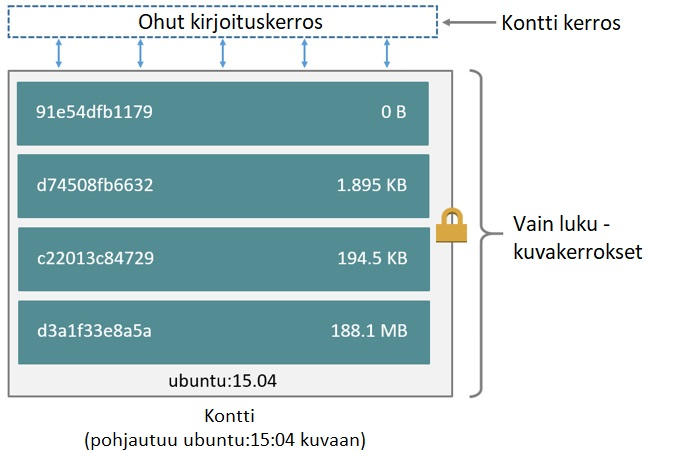
\includegraphics[width=1\textwidth]{images/container-layers.jpg}
        \caption{Dockerin kerroksista koostuva kuva. Huomaa vain yksi ohut kirjoituskerros \href{https://docs.docker.com/storage/storagedriver/\#images-and-layers}{(Docker 2018)}}
        \label{fig:container-layers}
    \end{figure}
    
    Tämän lisäksi Docker myös käyttää Advanced Multi-Layered Unification Filesystem (AuFS) kerrostettua tiedostojärjestelmää joka voi näkymättömästi kerrostaa useita tiedostojärjestelmiä päällekkäin. Sen avulla Docker voi jakaa samaa monen kontin käyttämää tiedostokerrosta vain luku -muodossa kaikille sitä tarvitseville konteille. Kontille itselle tarjotaan vain ohutta omaa kirjoitettavaa kerrosta joka on nopea luoda. Kontit kuitenkin suositellaan luotavan ilman kirjoituskerrosta eli tilattomana ja mahdolliset levylle kirjoittamiset tehtävän vain kontille varta vasten tarjottuun levy-asemaan. Tilattomia kontteja on moninverroin helpompi kehittää ja korjata. AuFS:in copy-on-write tiedostojärjestelmä tarjoaa myös helpon tavan seurata tiedostomuutoksia samaan tapaan kuin Git:in \texttt{diff} \cite{docker}.
    
    Ongelmia AuFS:n käytössä tuo sen hitaus verrattuna tavalliseen tiedostojärjestelmään. Myös kerroksittainen kirjoittaminen kasvattaa kontteja ajan kanssa jolloin on tarpeen niiden ajoittainen uudelleenluonti kerroksien yhdistämiseksi \cite{containers-in-multi-user-environments}.
    
    Docker ja muut kontit käyttävät myös monia eri kirjastoja paremman eristyksen ja turvallisuuden takaamiseksi kuten SELinux tai AppArmor \cite{practical-container}.
    
    \subsection{Kontit virtuaalikoneisiin verrattuna}
    
    Kontit tarjoavat virtuaalikoneisiin verrattuna kevyemmän virtuaalisaation ja nopeamman tavan luoda ja käynnistää uusia instansseja. Ehkä tärkeimpänä ominaisuutena kuitenkin voidaan pitää konttikuvia jotka mahdollistavat helpon tavan luoda ja muokata kontteja esimerkiksi juuri Dockerin ylläpitämän rekisterin DockerHubin kautta \cite{docker}. Tämä modulaarisuus hajautetuissa järjestelmissä on verrattavissa olio-ohjelmoinnin yleistymiseen 90-luvulla. Standardiyksikön kuten kontin käyttö mahdollistaa tehokkaamman systeemien hallinnan ja yleisten suunnittelumallien käytön \cite{container-design-patterns}.
    
    Kontit myös mahdollistavat helpomman tavan luoda mikropalveluarkkitehtuureja jossa ison monoliittisen sovelluksen sijaan logiikka on hajautettu omiksi erillisiksi palveluiksi \cite{practical-container, container-design-patterns}. Tämä tuo etuja sovelluksen ylläpidossa ja kehittämisessä kun eri osia voi vaihtaa sekä kehittää toisista riippumatta mikä myös tekee siitä skaalautuvamman \cite{goto-netflix}.
    
    \begin{figure}[h]
        \centering
        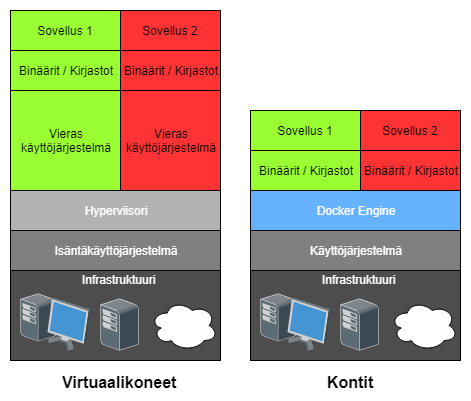
\includegraphics[width=1\textwidth]{images/Container-vs-VMs.png}
        \caption{Virtuaalikoneiden ja konttien virtuaalisaation ero \href{https://techglimpse.com/docker-installation-tutorial-centos/}{(Tech Glimpse 2017)}}
        \label{fig:c-vs-vm}
    \end{figure}
    
    Virtuaalikoneilla on kontteihin verrattuna etuna parempi käyttöjärjestelmätason eristys ja ne pystyvät käyttämään kehittyneempiä eristyksen muotoja kuten Intelin VT tai AMD-V \cite{openvz-xen-kvm}. Intelin VT teknologia mahdollistaa erilaisia tehokkuusparannuksia virtualisointiin. VT-x esimerkiksi antaa prosessorille 10 uutta konekäskyä \cite{vt-x-overview} ja moodin jolla vieraskäyttöjärjestelmä voi suorittaa ytimen tasolla 0 isäntäkäyttöjärjestelmän ollen yhä samalla suojattu \cite{vt-x-analysis}. AMD-V tuo samanlaisia lisäominaisuuksia prosessorille joka tehostaa virtualisoitujen komentojen suorittamista \cite{amd-v-snippet}.
    
    \subsection{Konttien ja virtuaalikoneiden tehokkuusvertailu}
    
    Konttien ja virtuaalikoneiden välisiä tehokkuuseroja on tutkittu jonkin verran mutta tuloksia on ollut vaikea tulkita virtuaalisaatioiden erilaisten ominaisuuksien takia. \textit{Measuring Docker Performance: What a mess!!!} (2017) -tutkimuspaperin mukaan lopullista päätelmää on vaikea antaa koska esimerkiksi ei ole olemassa tarpeeksi laajoja tai vakaita työkaluja konttien suorituskyvyn testaukseen \cite{docker-mess}. 
    
    Aiheesta hivenen vanhemmassa tutkimuspaperissa, \textit{Containers and Virtual Machines at Scale: A Comparative Study} (2016), tullaan johtopäätökseen että virtuaalikoneiden ja konttien välillä on tehokkuuseroja, mutta nuo erot selittyvät enemmän virtuaalisointien erilaisuudesta kuin toisen virtualisaation paremmuudesta. Kontit hyötyvät suorista kutsuista suoraan käyttöjärjestelmän ytimeen sekä pienemmästä koosta mutta samalla myös kärsivät heikommasta eristyksestä. Virtuaalikoneilla on tarkat resurssirajat kun taas kontit voivat hyödyntää muiden konttien vapaana olevia resursseja löysemmillä rajoituksilla. Tämän vuoksi yksi suosittu tapa ajaa kontteja on virtuaalikoneiden sisällä näin hyödyntäen virtuaalikoneen turvallisuutta ja samalla käyttäen konttien avulla kaikkia resursseja tehokkaasti hyväksi. Kehitteillä on myös uusi virtuaalikonetyyppi, kevyt virtuaalikone (lightweight VM),  jonka tarkoituksena olisi toteuttaa konttien ominaisuudet virtuaalikoneiden eristyksellä \cite{containers-vms-study}.
    
    \section{Konttienhallintajärjestelmät}
    
    \subsection{Johdanto}
    
    Internetin yleistyessä ja teknologian kehityksen kiihtyessä ovat resurssit palvelimien käytössä kasvaneet huomattavasti vuosikymmenten aikana. Esimerkiksi yksi Googlen uusi palvelinsali koostuu neljästä jalkapallokentällisestä ja kahdensadan miljoonan euron edestä palvelimia \cite{borg-goto-youtube}. Yksi suurista ongelmista valtavan palvelinmäärän hallinnassa on niiden resurssien optimointi mahdollisimman tehokkaasti. Google on ollut edelläkävijä tässä optimoinnissa ja he ovat kehittäneet järjestelmiä, joiden avulla he ovat huomattavasti parantaneet palvelimiensa käyttöastetta \cite{borg-omega-kubernetes}.
    
    Näistä järjestelmistä ensimmäinen oli Borg joka luotiin vuosina 2003-2004 korvaamaan joitain Googlen sisäisiä palveluita kuten Babysitter ja Global Work Queue, jotka olivat luotu hoitamaan pitkäaikaisia palveluita ja sarja-ajoja. Borgin tarkoituksena oli tehostaa resurssien käyttöä jonka mahdollisti konttimaisten ominaisuuksien kuten \texttt{cgroup}:in tulo Linuxin ytimeen, johon Google oli isolta osin vaikuttamassa. Sen käytön kasvaessa sitä kehitettiin palvelemaan montaa eri Googlen sisäistä tiimiä ja sille luotiin laaja määrä työkaluja sekä palveluita helpottamaan sen käyttöä
    \cite{borg-omega-kubernetes}.
    
    Borg toi kustannushyötyjä muun muassa käyttämällä jo varattuja mutta käyttämättömiä palvelinresursseja muihin lyhytaikaisiin sarja-ajoihin. Siinä ei myöskään haluttu maksaa virtuaalikoneiden aiheuttamia tehokkuusmenetyksiä joten useimmiten ohjelmat ajettiin Borgissa laitteistotasolla käyttäen kuitenkin konttimaisia eristyskeinoja prosessien eristämiseen. Tämä ei ole kuitenkin verrattavissa täyteen konttitotetukseen kuten Dockeriin \cite{management-with-borg}.
    
    Keskitetty hallintajärjestelmä myös mahdollisti kehittäjien keskittymisen pelkästään sovellusten kehittämiseen jättäen laitteistoriippuvuuksien ja aikatauluttamisen järjestelmän hoidettavaksi. Tämä muutti kehityksen laite-orientoituneesta sovellus-orientoituneeksi \cite{borg-omega-kubernetes}.
    
    Kuitenkin Borgin käytössä havaittiin pian ongelmia, joiden vuoksi ryhdyttiin luomaan uutta konttienhallintajärjestelmää näiden puutteiden korjaamiseksi. Syntyi Omega, jonka tarkoituksena oli edistää resurssien käyttöä tehokkaammalla aikatauluttajalla (scheduler). Borgin monoliittisen aikatauluttajan sijaan Omegassa se oli hajautettu moneksi erilliseksi aikatauluttajaksi joilla kaikilla oli pääsy klusterin Paxos-pohjaiseen tilaan. Tämä mahdollisti monipuolisempien aikataulutus-algoritmien käytön ja näin ollen tehokkaamman resurssien hyödyntämisen \cite{omega}.
    
    Omega ei kuitenkaan lopulta korvannut Borgia mutta monet sen innovoimista ratkaisuista lisättiin takaisin Borgiin ja käytettiin perustana Googlen seuraavan järjestelmän, Kuberneteksen, luomiseen.
    
    Kubernetes luotiin aikana jolloin ulkopuolinen kiinnostus kontteja ja konttienhallintajärjestelmiä kohtaan oli kiihtymässä ja Google tarjosi jo omaa kasvavaa pilvipalvelua Google Cloud Platform:ia (GCP). Edellisistä järjestelmistä poiketen Google päätti luoda Kuberneteksen alusta alkaen avoimen lähdekoodin projektiksi joka olisi Borgia kehittäjäystävällisempi sekä korjaisi joitain sen puutteita kuten yhtä IP-osoitetta per laite sekä töiden jakamista joustavammalla tavalla \cite{borg-omega-kubernetes}.
    
    Kubernetes on jatkuvassa määrin muodostumassa samanlaiseksi avoimen lähdekoodin standardiksi konttienhallintajärjestelmissä kuten Linux on käyttöjärjestelmille. Cloud Native Computing Foundation (CNCF), johon suurimmat teknologiayhtiöt kaikki kuuluvat, hyväksyi standardoidun Kuberneteksen API:n jonka jokainen jäsen on velvoitettu toteuttamaan omassa Kubernetes-pohjaisessa konttienhallinta-palvelussa \cite{kubernetes-cncf-standard-announcement}.
    
    Näiden lisäksi on monia muita konttienhallintajärjestelmiä kuten DockerSwarm, Mesos ja OpenStack mutta joista Docker ja MesosSphere ovat jo luvanneet tukensa Kubernetekselle kuten moni muukin pilvipalveluntarjoaja \cite{practical-container}.
    
    Jotta järjestelmien kehityskulku selventyisi käyn läpi näiden järjestelmien kehittymisen ja toiminnallisuuden vertailun.
    
    \subsection{Borg}
    
    Borg syntyi Googlen sisällä korvaamaan sisäisiä sovelluksia kuten BabySitter ja Global Work Queue, joilla hallittiin pitkäaikaisia prosesseja ja sarja-ajoja. Sen tarkoituksena oli yhtenäistää ja tehostaa resurssien käyttöä Googlen palvelimilla pakkaamalla suoritettavia prosesseja paremmin ja käyttämällä kehittyneitä aikataulutus-metodeja.
    
    Alussa Borg toimi suoraan palvelimien päällä ilman virtualisointia tehokkuuden maksimoimiseksi. Kuitenkin käyttöjärjestelmäriippuvuudet ja eri ohjelmistoversioiden hallinta teki kehittämisestä ajoittain vaikeaa kuten IBM huomasi jo aikoinaan.
    
    \begin{figure}[h]
        \centering
        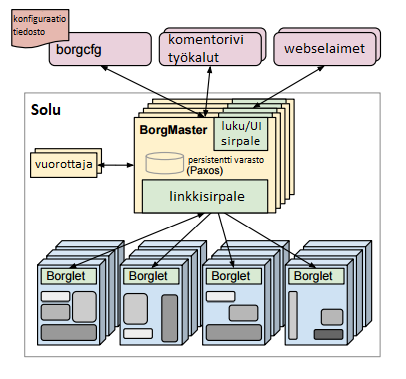
\includegraphics[width=1\textwidth]{images/borg.png}
        \caption{Borg kaavio Googlen julkaisemasta paperista. Linkkisirpale huolehtii kommunikaatiosta Borglettien välillä \href{https://ai.google/research/pubs/pub43438}{(Google 2015)}}
        \label{fig:borg}
    \end{figure}
    
    Borgin keskiössä on BorgMaster-palvelin joka hallinnoi koko klusteria. Yksittäinen klusteri joita kutsutaan myös soluiksi (cell) koostuu Googlella keskimäärin 10 000 palvelimesta. BorgMaster on replikoitu viidelle kopiolle jotka pitävät yllä viimeisintä kopiota klusterin tilasta ja joista valitaan uusi pääsolmu nykyisen kaatuessa. Kiireinen BorgMaster käyttää 10-14 prosessoriydintä ja 50 GiB RAM-muistia.
    
    Eräs esitys Borgin arkkitehtuurista on kuvattu kuvassa \ref{fig:borg}. Klusteri koostuu solmuista (node) jotka vastaavat yksittäistä fyysistä tai virtuaalista palvelinta. Solmun sisällä palvelimen resurssit ovat varattu allokaatioiksi (alloc, lyhenne sanasta allocation) ja sillä suoritetaan vähintäänkin Borglet-prosessia. Borglet-prosessi suorittaa sille annettuja tehtäviä allokaatioissa ja raportoi tilaansa BorgMasterille.
    
    Ensimmäiset Borgin versiot käyttivät yksinkertaista synkronista silmukkaa joka hyväksyi pyynnöt, aikataulutti tehtävät ja kommunikoi Borglettien kanssa. Solujen kasvaessa tämä pilkottiin omaksi palveluksi joka on replikoitu kuten pääsolmu ja joka koko ajan hakee uusinta tilaa pääsolmusta, päivittää kopionsa, aikatauluttaa tehtäviä ja raportoi pääsolmua noista muutoksista. Pääsolmu sitten hyväksyy tai hylkää muutokset jos ne perustuvat vanhentuneeseen tilaan. Tämä muistuttaa hyvin paljon Omegan optimistista samanaikaisuudenhallintaa johon se osaltaan perustuu.
    
    Tehtävä (task) on yksittäinen suoritettava ohjelma joka annetaan samanlaisena kaikille sille varatuille solmuille. Borg yrittää maksimoida juurikin tehtävien ajon mahdollisimman tehokkaalla tavalla. Suoritettavat tehtävät ovat Borgissa eristetty toisistaan konttimaisilla keinoilla kuten nimiavaruuksilla vaikka ne ei välttämättä käyttäisikään varsinaisia kontteja kuten Dockeria.
    
    Tehtävät taas kuuluvat aina yhteen työhön (job) joka annetaan BorgMasterille suoritettavaksi RPC-rajapinnan kautta niitä varten luodussa BCL-kielisessä konfiguraatiotiedostossa joka muistuttaa Dockerfileä. Se kuvaa kaiken työn suoritukseen tarvittavan tiedon ja se tallennetaan Borgin Paxos-varastoon ja jonka suorituksen kulkua BorgMaster koko ajan päivittää.
    
    Eräs Borgin ongelmallisuutta kuvaava ominaisuus on ollut mahdollisuus ajaa tehtäviä allokaatioiden ulkopuolella, jonka on kerrottu olleen syynä suureen määrään harmia: \textit{``Borg also allows top-level application containers to run outside allocs; this has been a source of much inconvenience.``}
    
    Ehkä kuitenkin tärkein osa Borgia on sen sisäinen logiikka resurssien mahdollisimman tehokkaaseen käyttöön erilaisten keinojen avulla kuten tiiviimpi ohjelmien pakkaaminen (bin packing), kapasiteetin hyödyntäminen ajamalla lyhytaikaisia sarja-ajoja jo varatuilla mutta vähän käytetyillä resursseilla sekä optimoitu resurssien varaaminen sovittaen ajettavat tehtävät niille sopiville solmuille. Googlen mittakaavassa nämä tehokkuusparannukset tuovat jo huomattavia kustannusvähennyksiä.
    
    Esimerkkejä palveluista joita Borgilla on ajettu ja yhä ajetaan on Googlen hakupalvelu, Google Docs ja Gmail. Borg on edelleen Googlen sisällä käytetyin klusterinhallintajärjestelmä ja sen monimutkaisuus mahdollistaa myös töiden monipuolisen konfiguroinnin mikä ei välttämättä Kuberneteksessa olisi mahdollista \cite{management-with-borg}.
    
    Ongelmiksi Borgissa on muodostunut esimerkiksi tehtävien ryhmittely pelkkien töiden avulla. Käyttäjä ei voi erotella tuotanto- ja testiympäristöä toisistaan muuten kuin luovilla nimeämisratkaisuilla. Tämä on johtanut taas työkalujen luontiin jotka parsivat nimistä laajemman palvelintopologian, mikä taas on tuottanut lisää monimutkaisuutta järjestelmään \cite{borg-goto-youtube}.
    
    Toinen iso ongelma on ollut yhden IP-osoitteen rajoite laitetta kohti. Borgissa samalla laitteella olevat tehtävät jakavat kaikki saman IP-osoitteen joten ne myös jakavat porttiavaruuden. Näin ollen Borgin tulee allokoida ja käsitellä niitäkin resursseina joita tulee varata ja vapauttaa. Tehtäviä jotka käyttävät samaa porttia kuten 80 ei voida näin ollen ajaa samalla laitteella muuttamatta niiden konfiguraatiota.
    
    Kolmas iso ongelma on ollut Borgin optimointi tehokäyttäjille tavallisten käyttäjien kustannuksella. Borg tukee laajan määrän eri konfiguraatio-asetuksia monille vaativille Googlen sisäisille palveluille joka tekee sen API:n kehityksestä vaikeaa. Ratkaisuna on ollut työkalujen luonti jotka automatisoivat ja hallinnoivat näitä käyttäjän puolesta.
    
    Hyvinä puolina kuitenkin on huomattu kuinka käytännöllisiä allokaatiot ovat olleet, miten klusterin hallinta on enemmän kuin tehtävien hallintaa ja että introspektio, jälkihavainnointi, on hyvin tärkeää \cite{management-with-borg}.
    
    \subsection{Omega}
    
    Ajan saatossa ja Borgin kasvaessa yhä monimutkaisemmaksi havaittiin sen käytössä joitain ongelmia joita Google halusi ratkaista. Borgissa ajettava kuorma oli hyvin vaihtelevaa, joten sen mahdollisimman tehokas aikatauluttaminen vaati monipuolisia ominaisuuksia Borgin monoliittiselta aikatauluttajalta. Tämä monimutkaisuus oli kuitenkin muodostumassa yhä vaikeammaksi hallita ja osana sen uudelleenkirjoitusta Google päätti tutkia uudenlaista tapaa lähestyä ongelmaa \cite{omega}. Tavoitteena oli myös parantaa Borgin ohjelmistolaatua sen koostuessa monesta eri ad hoc -tapaan liitetystä palvelusta \cite{borg-omega-kubernetes}.
    
    Tätä varten luotiin uusi konttienhallintajärjestelmä, Omega, jonka keskiössä oli halu kehittää täysin uusi aikatauluttaja tehostamaan palvelimien käyttöastetta. Toisin kuin Borg, jossa yksi monoliittinen aikatauluttaja huolehti kaikista muutoksista, Omegan aikatauluttaja perustui jaettuun tilaan, jolloin monella eri aikatauluttajalla oli mahdollisuus päästä tilaan samanaikaisesti käsiksi. Tämän avulla kaikkea logiikkaa ei tarvinnut lisätä yhteen vuorottajaan, vaan algoritmit voitiin jakaa eri vuorottajiin jotka puolestaan kilpailivat resurssien vuorottamisesta.
    
    Mahdolliset yhteentörmäykset vuorottajien välillä tilaa päivittäessä hoidettiin optimistisella samanaikaisuudenhallinnalla (optimistic concurrency), jolloin kaikki vuorottajat pääsevät käsiksi kaikkiin resursseihin ja konfliktien sattuessa ne havaitaan jälkeenpäin ja muutokset perutaan. Pessimistinen hallinta lukitsisi resurssit jokaisella vuorottajalle yksi kerrallaan joka estää päällekkäiset muutokset, mutta hidastaa vuorottajien toimintaa.
    
    Tämä uusi aikataulutustapa on sittemmin tehty myös Borgiin ja sen pohjalta on myös rakennettu Googlen seuraava konttienhallintajärjestelmä Kubernetes \cite{omega}.
    
    \subsection{Kubernetes}
    
    Toisin kuin aikaisemmat Googlen järjestelmät luotiin Kubernetes alun pitäen avoimen lähdekoodin projektiksi. Sen tarkoitus oli luoda kehittäjä- ja käyttäjäystävällisempi versio Borgista, joka korjaisi myös joitain Borgissa havaittuja puutteita. Se esimerkiksi pakottaa hyvin yhtenäisen rajapinnan toisin kuin Borg, jonka rajapinta oli hitaasti kasvanut vuosien aikana hyvin monimutkaiseksi \cite{borg-omega-kubernetes}.
    
    Kuberneteksen kehitys aloitettiin vuonna 2014 ja annettiin Linux Foundationin hallinnoivan Cloud Native Computing Foundation:n alaisuuteen vuonna 2015 \cite{tc-kubernetes-cncf}. Kuberneteksessä ja Borgissa on hyvin paljon yhteistä ja sitä voidaan tavallaan katsoa kevyemmäksi versioksi Borgista \cite{borg-goto-youtube}.
    
    \begin{figure}[h]
        \centering
        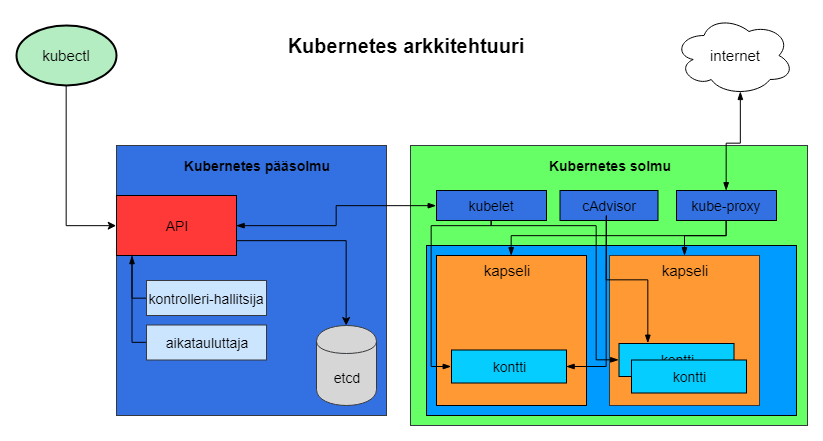
\includegraphics[width=1\textwidth]{images/kubernetes-2.png}
        \caption{Yksinkertaistettu näkymä Kuberneteksen toiminnasta \href{https://www.youtube.com/watch?v=YKg7uNMy_rc}{(Rock Mutchler 2017)}}
        \label{fig:kubernetes}
    \end{figure}
    
    Kuberneteksen arkkitehtuuri on kuvattu kuvassa \ref{fig:kubernetes}. Yksi Kubernetes klusteri koostuu yhdestä pääsolmusta (master node) joka on useimmiten replikoitu monelle eri datakeskukselle häiriöiden varalta. Tämän on hyvin samankaltainen Borgiin verrattuna ja pääsolmulle myös voidaan lähettää pyyntöjä joko sen HTTP- tai RPC-rajapinnan kautta tai suoraan kubectl-hallintasovelluksella.
    
    Pääsolmu hallitsee klusterin tilaa etcd\footnote{\url{https://coreos.com/etcd/}} avain-arvo-varastossa ja varaa sekä hallitsee resursseja käyttäjän tekemän konfiguraation mukaisesti. Erona Borgiin ja Omegaan on konsensus-algoritmi, joka niissä on Paxos, Kuberneteksessä Raft.
    
    Kuten Borgissa klusteri koostuu Kuberneteksessä solmuista (node) jotka vastaavat joko fyysisiä tai virtuaalisia palvelimia. Yksittäinen solmu sisältää ainakin Kubelet-hallintaprosessin sekä konttien konttienhallintaohjelman kuten Dockerin.
    
    Solmun sisällä taas on joukko kapseleita (pod) jotka koostuvat yhdestä tai useammasta kontista. Yleinen käytäntö on pitää vain yhtä konttia per kapseli paitsi jos kyseessä on tiukasti toisiinsa sidottu palvelu kuten webpalvelin ja lokientallennussovellus.
    
    Kapselit ovat Kuberneteksen atominen yksikkö ja ovat verrattavissa Borgin allokaatioihin. Ne ovat tarkoitettu olemaan hetkellisiä ja jatkuvasti muuttuvia joita Kubernetes hallinnoi käyttäjiensä puolesta kuten miten kapselit jaetaan eri solmuille. Saman kapselin sisällä kontit jakavat levyn ja verkkoavaruuden joten kontit voivat löytää toisensa \texttt{localhost}:in avulla. Erona Borgiin jokaisella kapselilla on oma uniikki IP-osoite joten kontit sen sisällä voivat käyttää portteja miten haluavat.
    
    Kapseleita ei suositella luomaan suoraan vaan niitä varten luotujen kontrollerien avulla jotka kuvaavat kapselin ajamiseen tarvittavat tiedot. Esimerkiksi korkeamman tason Deployment-kontrolleri on normaali tapa kuvata yhtä kapselia ja määrittämään esimerkiksi kuinka monta kapselia pidetään jatkuvasti käynnissä ja miten niiden määrää muutetaan kuormituksen kasvaessa tai laskiessa. StatefulSet-kontrolleria suositellaan käytettävän kapseleihin jotka ylläpitävät tilaa kuten tietokannat ja joka takaa hallitun tilan siirron vanhoista versioista uusiin. Deploymentin lisäksi useimmat kapselit toteuttavat myös vähintäänkin ReplicaSet:in jonka avulla tietty määrä kapseleita pidetään aina käynnissä niiden kaatuessa sekä skaalataan ylös tai alas kuorman muuttuessa.
    
    Kapseleille voidaan myös antaa muita ominaisuuksia erilaisten abstraktioiden avulla. Service avaa kapselista portin ulos ulkopuoliseen internettiin ja sitä käyttävät kapselit valitaan selektorien (selector) avulla joilla on tietty nimike (label). Kuberneteksen konfiguraation kirjoittamiseen käytetään YAML-tiedostoja \cite{kubernetes-docs}.
    
    Optimoidun resurssienhallinnan lisäksi isoin etu Kuberneteksen kaltaisessa palvelimien hallintajärjestelmässä on riippumattomuus palvelininfrastruktuurista. Kubernetes-klusteri on mahdollista ajaa omilla palvelimilla yhtä lailla kuin pilvessä kuten AWS:ssä tai GCP:ssä ilman suurempaa konfiguraation uudelleenkirjoittamista \cite{kubernetes-rule-world}.
    
    Kubernetes voidaan nähdä esimerkkinä koreografiasta, jossa joukko itsenäisiä mikropalveluita ja pieniä kontrollisilmukoita luo yhteistyössä emergentin kokonaisuuden. Se on vastakohta keskittyyn orkestrointiin joka on helpompi luoda alussa, mutta joka myöhemmin muodostuu herkäksi ja kankeaksi erityisesti odottomattomien virheiden ja tilamuutosten takia \cite{borg-omega-kubernetes}.
    
    \subsection{Edut ja ongelmat}
    
    Laajamittaisella konttien hallinnoimisella on mahdollista ylläpitää valtavia määriä palvelimia joka muilla tavoin tuskin olisi mahdollista. Kuitenkin konttihallintajärjestelmissä on edelleen ongelmina muun muassa konfiguraatio ja riippuvuuksien hallinta.
    
    Yhden suuren ympäristön konfiguraatio on vaikeaa ja vaatii nopeasti oman Turing-vahvan kielen. Ratkaisu on selkeästi erottaa data ja laskenta toisistaan jolloin staattinen informaatio on jossain formaatissa kuten JSON tai YAML ja laskenta tuotetaan jollain ohjelmointikielellä jolla on hyvin tunnettu semantiikka ja virheenkorjaustuki.
    
    Uuden palvelun käynnistäminen usein vaatii monen muun eri palvelun käynnistämistä (monitorointi, tiedostovarasto, CI/CD) joiden keskinäisiä riippuvuuksia on useimmiten mahdoton pitää yllä automaattisesti. Näiden riippuvuuksien rekisteröinti ja hallitseminen tekee kehittämisestä vaikeaa ja usein johtaa siihen, että parhaita käytäntöjä ei noudateta. Tämä riippuvuuksien hallinta on yhä avoin ongelma konttienhallintajärjestelmien kanssa \cite{borg-omega-kubernetes}.
    
    \section{Suunnittelumalleista}
    
    Konttien standardiominaisuuksien takia sille on muodostunut erilaisia käyttötapoja joita voi luonnehtia suunnittelumalleiksi (design pattern). Yleisin tapa konteille on tietenkin luoda ne yksittäisinä kokonaisuuksina ilman erillisiä riippuvuuksia toisiin kontteihin kuten tietokantapalvelin tai monoliittinen applikaatiopalvelin.
    
    \subsection{Yhden solmun, usean kontin malleja}
    
    Sivuvaunu (sidecar) -mallissa on yksi pääkontti ja toinen pääkonttia tehostava kontti joka huolehtii tietystä tehtävästä pääkontin puolesta. Eräs esimerkki on webpalvelin ja sen lokeja levyltä hakeva ja tallentava lokitallentaja-palvelu. Toinen esimerkki on webpalvelin ja kontti, joka jatkuvasti synkronisoi webpalvelimen tarjoamaa sisältöä Git:in tai jonkin muun datalähteen kautta.
    
    Hyötyinä kahden kontin käyttö yhden kontin sijaan on tässä tapauksessa resurssien tehokkaampi allokointi jolloin webpalvelin saa käyttöönsä isoimman osan resursseista ja lokitallentaja hyödyntää loppuja kun webpalvelin ei niitä tarvitse. Palvelua on myös helpompi käsitellä kahtena eri kokonaisuutena ja kehittää toisista erillään. Lokitallentajaa on tällöin myös mahdollista käyttää toisten konttien kanssa.
    
    Eräs toinen malli on suurlähettiläs (ambassador) -malli jossa pääkontin kommunikointi johonkin toiseen palveluun on välitetty toisen kontin lävitse. Näin pyyntö voidaan esimerkiksi hajauttaa taustalla olevaan tietokantaklusteriin pääkontin siitä tietämättä helpottaen pääkontin sovelluksen kehittämistä.
    
    Sovitin (adapter) -malli on samanlainen suurlähettiläs-malliin verrattuna mutta missä suurlähettiläs esittää yksinkertaistetun näkymän pääkontille, sovittimessa pääkontti esitetään ulkopuoliselle maailmalle yksinkertaistettuna näkymänä. Näin voidaan esimerkiksi muuntaa erilaiset monitorointi-rajapinnat samaksi yhtenäiseksi rajapinnaksi koko klusterin sisällä \cite{container-design-patterns}.
    
    \subsection{Monen solmun malleja}
    
    Siirryttäessä yhdellä palvelimella toimivista konttimalleista monen solmun malleihin, selventävät kontit niiden luontia yksinkertaisilla rajapinnoilla, joita järjestelmän osat toteuttavat.
    
    Yleinen ongelma hajautetuissa järjestelmissä on johtajan valinta monesta samanlaisesta kopiosta. Johtajan valinta (leader election) -mallissa voidaan erilaisten linkitettävien kirjastojen käytön sijaan käyttää valitsija-konttia, jonka kanssa keskustelevat kopiot toteuttavat jonkin rajapinnan tietojen lähettämiseen valitsija-kontille. Valitsija-kontin voi luoda aiheeseen erikoistunut asiantuntija ja kehittäjät uudelleenkäyttää sitä välimättä siitä, millä ohjelmointikielellä se on toteutettu.
    
    Työjono (work queue) on myös toinen yleinen malli hajautetuissa järjestelmissä ja siihen on monia eri kehysmalleja (framework) mutta jotka pakottavat kehittäjän tiettyyn ohjelmointikieleen tai alustaan. Konttien avulla kehittäjä voi luoda kontin, joka toteuttaa halutut kehysmallin vaatimat rajapinnat kuten \texttt{run()}- ja \texttt{mount()}-metodit. Tämän kontin tehtävänä on sitten vain ottaa vastaan syöte-tiedostoja tiedostojärjestelmästä ja muuntaa ne ulostulo-tiedostoksi. Kaiken muun työjonoon liittyvän voi valmis kehysmalli huolehtia eriyttäen vain prosessoivat osat kontteina erilleen.
    
    Viimeisenä esiteltävänä mallina on hajoittaja-kerääjä (scatter/gatherer) -malli jossa ulkopuoliset asiakasohjelmat (client) lähettävät pyyntöjä juurisolmulle (root node). Tämä juurisolmu taas lähettää pyyntöjä sille allokoiduille palvelimille, jotka suorittavat laskennan rinnakkaisesti. Jokainen pirstale (shard) palauttaa osittaisen datansa juurelle, joka kerää vastaukset yhdeksi vastaukseksi asiakkaalle. Tämä malli on yleinen hakukoneissa. Iso osa sen toteutusta koostuu geneerisistä osista jotka voidaan konteilla luoda tiettyjen rajapintojen toteuttaviksi osiksi, mikä yksinkertaistaa sen rakennetta \cite{container-design-patterns}.
    
    \section{Pilvipalvelujen tarjoajista}
    
    \subsection{Johdanto}
    
    Konttipohjaisten ratkaisujen yleistyessä monet pilvipalvelujen tarjoajat keskittyvät yhä etenevissä määrin tarjoamaan niille räätälöityjä ratkaisuja. Googlen pilvipalvelu GCP (Google Cloud Platform) on yksi pisimpään näitä palveluita tarjonnut yhtiö (2015) \cite{gcp-kubernetes} ja monet muut ovat seuranneet sitä kuten AWS (2017) \cite{aws-kubernetes}, Azure (2017) \cite{azure-kubernetes} ja DigitalOcean (2018) \cite{digital-ocean-kubernetes}.
    
    \subsection{AWS}
    \label{ch:aws}
    
    AWS (Amazon Web Services) on markkinaosuudeltaan suurin pilvipalveluntarjoaja (Amazon 34\%, Microsoft 11\%, IBM 8\% ja Google 5\%)\footnote{\url{https://www.srgresearch.com/articles/leading-cloud-providers-continue-run-away-market}} joka selittyy AWS:n oltua monia muita aikaisemmin markkinnoilla että sen jatkuvalla uusien palveluiden innovoimisella \cite{aws-leading-cloud}. AWS tarjoaa laajan valikoiman eri palveluita joista konttienhallintapalvelu on vain yksi osa.
    
    ECS (EC2 Container Service) on alkuperäinen AWS:n konttipalvelu joka tuli markkinoille vuonna 2015 \cite{aws-introducing-ecs}. Se on verrattavissa ehkä enemmän Borgiin kuin Kubernetekseen ja se on täysin hallittu AWS:n puolesta ja integroitu muihin AWS:n palveluihin. Käyttäjän tarvitsee vain luoda tehtäviä, joiden sisällä kontit ajetaan ja joita ECS aikatauluttaa klusterilla ajettavaksi. ECS:n konfiguraation voi tehdä joko konsolista, komentoriviltä tai AWS:n oman CloudFormation-palvelun kautta JSON tai YAML-tiedoistoilla. Nämä tiedostot soveltuvat vain AWS:n palveluihin \cite{aws-docs-ecs}.
    
    EKS (Elastic Kubernetes Service) on AWS:n uusi Kubernetes-palvelu joka vielä tätä tutkielmaa kirjoittaessa oli suljetussa testikäytössä eikä vapaasti kaikkien saatavilla. Se kuten Googlen palvelu on AWS:n omien palveluiden kanssa integroitu Kubernetes joka myös huolehtii automaattisesti pääsolmujen replikoinnista ja kestävyydestä. Verrattuna ECS:ään se on riippumaton AWS:stä ja sama Kubernetes klusteri tulisi olla mahdollista siirtää toiseen palveluntarjoajaan ilman suurempaa vaivaa \cite{aws-docs-eks}.
    
    AWS tarjoaa myös uudenlaista palvelitonta (serverless) kontti-palvelua nimeltä Fargate ECS:n tai EKS:n kanssa käytettäväksi. Fargaten avulla käyttäjä voi luoda kontteja joita ajetaan vain tarvittaessa. Näin ollen ne minimoivat hukkakäytön ja käyttäjä maksaa vain siitä ajasta, jolloin ne ovat käynnissä \cite{aws-docs-fargate}.
    
    ECR (Elastic Container Registry) on rekisteri Dockerkuvien tallentamiseen joka on syvästi integroitu ECS:n kanssa. Sen avulla käyttäjä voi pitää omaa täysin-hoidettua rekisteriään joka skaalautuu automaattisesti kuorman mukaan \cite{aws-docs-ecr}.
    
    \subsection{GCP}
    \label{sb:gcp}
    
    Google Cloud Platform (GCP) on Googlen pilvipalvelu jonka erikoisuutena ovat datan käsittelyyn erikoistuneet palvelut kuten TPU-palvelimet, BigTable ja MapReduce \cite{gcp-advantages}.
    
    GCP myös tarjoaa kehittynyttä Kubernetes-palvelua johtuen suuresti siitä, että kyseessä on isolta osin Googlen luoma järjestelmä. Muut pilvipalveluntarjoajat ovat jo kuitenkin osin kuroneet kiinni Googlen etumatkaa ja tarjoavat melkein yhtä kattavia palveluita \cite{kubernetes-competition}.
    
    Kubernetes Engine (KDE) on Googlen tarjoama hoidettu Kubernetes-palvelu joka integroituu muiden GCP:n palveluiden kanssa ja joka hyötyy Googlen omasta konttijärjestelmien hallintaan liittyvästä osaamista \cite{kde-docs}.
    
    \subsection{Hintavertailu}
    
    Hintojen vertailu eri palveluntarjoajien välillä on vaikeaa erilaisten palveluiden ja ratkaisujen takia. Useimmat palvelut käyttävät Kubernetes-solmuinaan normaaleja virtuaalikoneita joita on mahdollista saada edulliseen hintaan pitkäkestoisilla sopimuksilla.
    
    Cloud Spectator -nimisen pilvipalveluihin keskittyneen konsultointiyrityksen vuoden 2017 raportin mukaan sekä AWS että GCP ovat pelkillä virtuaalikoneiden tuntikustannuksilla mitattuna suhteellisen kalliita pienempiin tarjoajiiin verrattuna. Kuitenkin pitkäkestoisilla sopimuksilla niiden molempien hinnat ovat halvimmasta päästä varsinkin suurikokoisilla instansseille \cite{cloud-price-comparison}.
    
    Virtuaalikoneiden lisäksi tavallinen Kubernetes-klusteri käyttää myös virtuaalilevyä joista esimerkkinä ovat vaikkapa GCP:n Compute Engine Persistent Disks ja AWS:n Elastic Block Storage (EBS) voluumit sekä Elastic File System (EFS). Raportin mukaan AWS on yksi halvimpia virtuaalilevyjen tarjoajia ja esimerkiksi GCP:tä hivenen halvempi \cite{cloud-price-comparison}.
    
    Kuitenkin tavallinen suuri palvelinarkkitehtuuri käyttää monia eri palveluita joita hintavertailu ei ota huomioon.
    
    Tutkimus- ja neuvonta-yhtiö Gartnerin käyttäjien antamissa arvioissa AWS ja GCP ovat molemmat saaneet saman arvosanan 4.4 \cite{gartner-aws-gcp}.
    
    \section{Mielipiteitä konteista}
    
    Kontit ovat saaneet kritiikkiä ylimääräisen kompleksisuuden lisäämisestä sovelluksiin, jotka eivät välttämättä sitä tarvitse. Kontteja saatetaan käyttää mustan laatikon tavoin joiden käyttäytymistä ei kehittäjä täysin ymmärrä.\footnote{\url{https://news.ycombinator.com/item?id=16445467}}
    
    Moderni palvelimienhallinta on kuitenkin hiljalleen keskittymässä virtualisointi-pohjaisiin ratkaisuihin eikä kehitykselle ole syytä nähdä loppua. Monet ongelmat joita suoraan rautatasolla toimivissa palvelimissa esiintyy katoavat siirryttäessä virtualisoituun ympäristöön. 
    
    Ovatko tulevaisuuden palvelimet sitten virtuaalikone- vai kontti-pohjaisia? Kontit kapseloivat ympäristönsä erittäin helposti käytettävään ja kehitettävään muotoon, joka helpottaa palvelimien kehittämistä ja jakamista. Tämä yhdistettynä tehokkuuden ja eristettävyyden parannuksiin luovat hyvin houkuttelevan tavan kehittää moderneja palvelinratkaisuja. Näkisin että tulevaisuuden palvelin tulee olemaan kuvattu konttikuvana.
    
    Virtuaalikoneet eivät kuitenkaan kokonaan katoa vaikkakin ne eivät tavallisten kehittäjien työkuvaan liiemmin kuulu. Eristetyn ympäristön luominen palvelimille voidaan yhä toteuttaa vain virtuaalikoneella konttien turvallisuusongelmien takia joten pilvipalvelujentarjojat tuskin luopuvat niistä pääasiallisena toimintaympäristönä. Näkisin että ne toimivat parhaiten yhdessä täydentäen toisiaan, eivätkä ole toisiaan poissulkevia vaihtoehtoja.
    
    Kehittäjien siis olisi parempi oppia tuntemaan kontit paremmin ja toivoisinkin, että tulevaisuudessa tullaan tarjoamaan esimerkiksi Helsingin Yliopistossa enemmän opetusta konteista.
    
    \section{Yhteenveto}
    
    Käyttöjärjestelmätason virtualisaatio on vanha keksintö joka on viimein saanut muotonsa kontiksi kutsuttuna toteutuksena. Sen avulla voidaan palvelimia kuvata yksinkertaisella ja standardilla tavalla helpottaen hajautettujen järjestelmien kehittämistä. Kontit tarjoavat virtuaalikoneisiin nähden kevyemmän virtuaalisaation vaikkakin ne kärsivät turvallisuusongelmista. Käyttämällä konttienhallintajärjestelmää voidaan kontti-pohjaisten palvelinten käyttöastetta parantaa tehokkaalla aikataulutuksella ja kuormaan sopivilla algoritmeilla. Avoimen lähdekoodin konttienhallintajärjestelmä kuten Kubernetes mahdollistaa myös palvelimien siirron pilvipalveluntarjoasta toiseen tai omille palvelimille vähäisellä vaivalla.
    
    \nocite{*}
    % Pick reference list style
    % numbered, in alphabetic order
    \bibliographystyle{abbrv}
    
    
    % apastyle
    %apaciten kaverina tarvitaan alussa usepackage-rivi
    %\bibliographystyle{apacite} % toimii sellaisenaan babelbibin kanssa
    
    %\bibliographystyle{apalike} % ei toimi babelin kanssa
    
    % old ABC80 mnemonics
    %\bibliographystyle{tktl} % babelbibin mukainen
    % edellisissä versioissa bblj pakotettu In-muotoon
    
    %\bibliographystyle{babunsrt} % numbering citation order
    %\bibliographystyle{babplain}
    %\bibliographystyle{babacm}
    %\bibliographystyle{babieeetr}
    
    
    %\bibliographystyle{abbrv}
    \bibliography{lahteet}
    
    % \bibliography{lahteet-muistikkailla}
    
    % vaihtoehtona vielä vanha mnemoninen tyyli (muistikkaat)
    % Muistikastyylissä lähteen tunnisteena käytetään lyhennettä. joka
    % koostuu kolmesta kirjaimesta ja kahdestas numerosta. Kirjaimet ovat tekijän
    % tai tekijöiden sukunimien alkukirjaimia ja numerot vuosiluvun kaksi
    % viimeistä numeroa.
    
    \lastpage
    
    \appendices
    
    \pagestyle{empty}
    
    \end{document}